\documentclass[11pt, a4paper]{beamer}
\usetheme{default}
\useoutertheme{infolines}
\usepackage{graphicx}
\usepackage{hyperref}
\usepackage{latexsym}
\usepackage{amsfonts}

\title{Tweets Conceptualization and Classification}
% \subtitle{An Introduction for Word Embedding}
\author{WANG Yue\and{ywangby@ust.hk}}
\institute[HKUST]{
    Department of Computer Science \\
    Hong Kong University of Science and Technology \\
}
\date{\today}

% structure
% problem defination
% method

\begin{document}
% title page
\begin{frame}[plain]
    \titlepage
\end{frame}

\begin{frame}{Problem Defination}
Given a short piece of message such tweets, how to capture the semantic information of it, such as topic and subject information?
\end{frame}

% aim
\begin{frame}{Twitter Conceptualization Examples}
\begin{center}
    \begin{figure}
        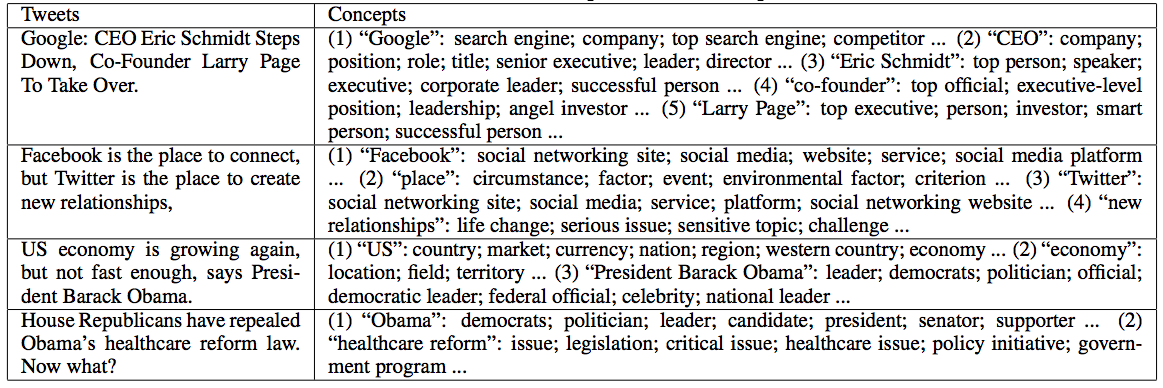
\includegraphics[width=1.0\textwidth]{./figure/tweets_concep_example.png}
        \caption{Tweets Conceptualization Example}
    \end{figure}
\end{center}
\end{frame}

% basic steps
\begin{frame}{Intuitive Steps in Tweets Clustering}
For each tweet:
\begin{enumerate}
    \item detect entities included in \textbf{knowledgebase}(longest entity)
    \item get the concepts of the entities in knowledgebase
    \item user the concept features to cluster the tweets
\end{enumerate}
\end{frame}

% basic description of knowledgebase
\begin{frame}{Description of Knowledgebase}
The taxonomy is a \textbf{directed acyclic graph}.
\begin{itemize}
    \item contains \textbf{isA} relationship
    \item \emph{concept} $\rightarrow$ \emph{instance}, \emph{attribute}(extract syntactic hearst patterns from webpages)
    \item claims in knowledgebase is associated with scores such as \emph{plausibility}, \emph{typicality}.
    \item each concept may have multiple senses(meanings)
    \item hierarchical structure
\end{itemize}
\end{frame}

% derive concepts of tweets based on knowledgebase
\begin{frame}{Derive Concepts Based on Knowledgebase}
Given a set of terms, how to derive their concepts.\\
Notation:
\begin{itemize}
    \item candidate concepts: $C = \{c_{k}, k \in 1,\cdots,K\}$
    \item terms are instances: $ E = \{ e_{i}, i \in 1,\cdots,M\}$
    \item terms are attributes: $ A = \{ a_{j}, j \in 1,\cdots,N\}$
    \item terms are unknown types: $ T = \{t_{l}, 1,\cdots,L\}$
\end{itemize}
\end{frame}

% naive bayes model
\begin{frame}{Derive Concepts: Naive Bayes Model}
When terms is a set of instances:
\begin{displaymath}
    P(c_{k} | E) = \frac{P(E|c_{k})P(c_{k})}{P(E)} \propto P(c_{k})\prod_{i = 1}^{M} P(e_{i} | c_{k})
\end{displaymath}
Where:
\begin{displaymath}
    P(e_{i} | c_{k}) = \frac{P(e_{i}, c_{k})}{P{c_{k}}}
\end{displaymath}
The concept with the largest posterior probability is ranked as the most possible concept to describe the observed instances. The process it similar to attrs and unknown terms.
\end{frame}

% how to build knowledge base
\begin{frame}{How to Construct Probabilistic Taxonomy and Knowledgebase}
\begin{columns}[T]
    \begin{column}{0.5\textwidth}
        \begin{center}
            \begin{figure}
                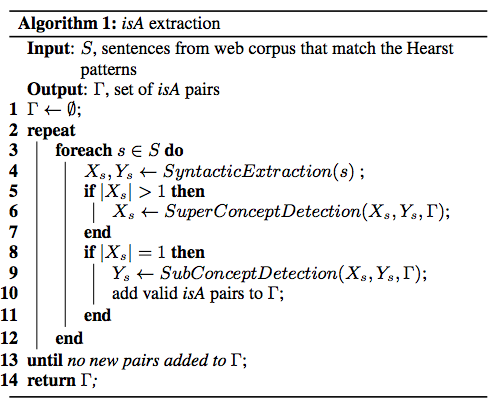
\includegraphics[width=0.8\textwidth]{./figure/is_a_extraction.png}
                \caption{\small{step 1: extract isA pairs from sentences}}
            \end{figure}
        \end{center}
    \end{column}
    \begin{column}{0.5\textwidth}
        \begin{center}
            \begin{figure}
                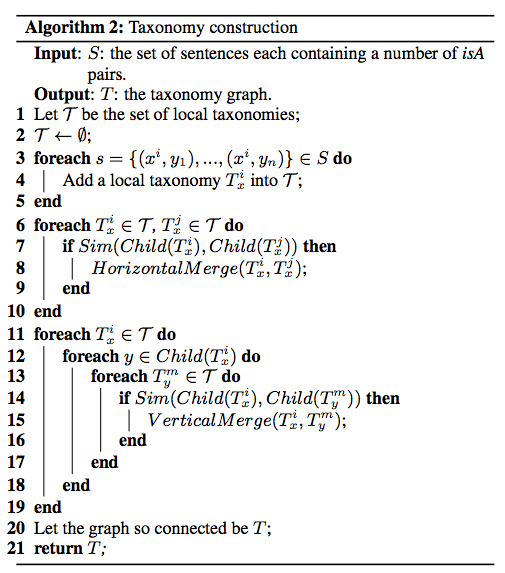
\includegraphics[width=0.8\textwidth]{./figure/taxonomy_construction.png}
                \caption{\small{step 2: construct the taxonomy as DAG}}
            \end{figure}
        \end{center}
    \end{column}
\end{columns}
\end{frame}

\end{document}
